\chapter{Analiza eksploracyjna}

\section{Zbiór danych - EmoContext}

Zbiór danych został udostępniony przez zespół z Międzynarodowych Warsztatów Ewaluacji Semantycznej (ang. \textit{SemEval-2019 International Workshop on Semantic Evaluation}) jako jedno z zadań konkursowych o nazwie EmoContext\footnote{\url{https://www.humanizing-ai.com/emocontext.html}} (ang. \textit{Contextual Emotion Detection in Text}).  Celem jest odkrycie prawidłowej etykiety emocji dla danego dialogu, składającego się z trzech wypowiedzi. W zadaniu tym użyty jest uproszczony model emocji zaproponowany przez Paula Ekmana \cite{ekman1993facial}, składający się z czterach klas: \textit{Happy}, \textit{Sad}, \textit{Angry} oraz \textit{Others}. Przykładowe dialogi oraz odpowiadające im etykiety emocji pochądzące ze zbioru treningowego zaprezentowane są na rysunku \ref{rys:examples_semeval}.

\begin{figure}[h]
\centering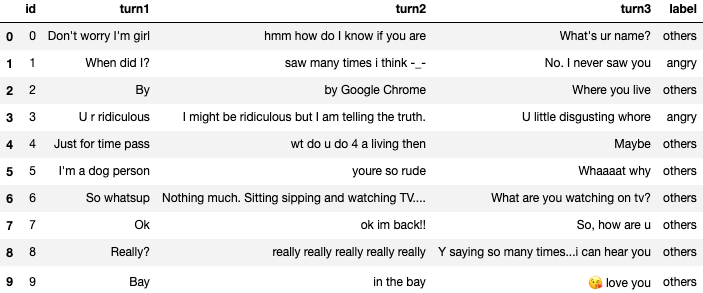
\includegraphics[width=12cm]{figures/examples_semeval.png}
\fcmfcaption{Przykładowe dialogi w danych z EmoContext wraz z etykietą emocji.}\label{rys:examples_semeval}
\end{figure}

\subsection{Szczegóły poszczególnych zbiorów}

Przez organizatorów konkursu udostępnione zostały następujące zbiory do ewaluacji własnych modeli: zbiór treningowy (\textit{train}), zbiór walidacyjny (\textit{dev}) oraz zbiór testowy (\textit{test}). Każdy z tych zbiorów zawiera tą samą strukturę danych, każdy przykład składa się z identyfikatora (\textit{Id}), trzech wypowiedzi w dialogu oraz etykiety emocji. Szczegółowe informacje na temat tych zbiorów ukazuje tabela \ref{tab:tabela_emocontext}.

\begin{table}[ht]
\fcmtcaption{Tabela prezentująca informacje o zbiorach w danych z EmoContext.}\label{tab:tabela_emocontext}
\centering\footnotesize%
\begin{tabular}{c c c}
\toprule
zbiór & liczba przykładów & najczęstsza klasa \\
\midrule
train   & 30160 & \textit{Others} 50\% \\
dev   & 2755 & \textit{Others} 84\% \\
test   & 5509 & \textit{Others} 84\% \\
\bottomrule
\end{tabular}
\end{table}

\subsection{Analiza zbiorów}

Aby lepiej zrozumieć dane treningowe przeprowadzone zostały podstawowe analizy eksploracyjne tego zbioru. Jedną z nich jest rozkład długości całego dialogu zaprezentowany na rysunku \ref{rys:rozklad_dl_semeval}. Widzimy na nim że przeważające dialogi są dosyć krótkie, średnio 62 znaki, co może utrudnić zadanie rozpoznania właściwej emocji. Zauważyć można także występujący długi ogon w kierunku coraz dłuższych dialogów, najdłuższy z nich ma 692 znaki.

\begin{figure}[t]
\centering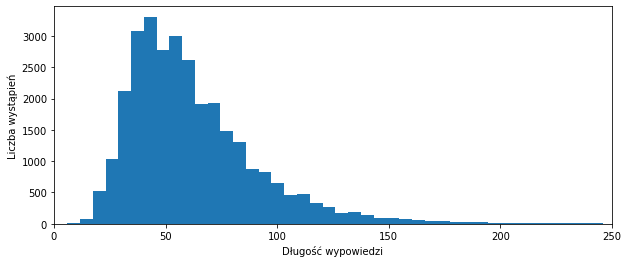
\includegraphics[width=12cm]{figures/rozklad_dl_semeval.png}
\fcmfcaption{Rozkład długości dialogu w danych z EmoContext.}\label{rys:rozklad_dl_semeval}
\end{figure}

Kolejna analiza to histogram częstości występowania danej etykiety w zbiorze treningowym, dzięki temu można sprawdzić czy występuje niezbalansowanie klas. Rysunek \ref{rys:rozklad_liczby_klas_semeval} prezentuje dominację klasy \textit{Others} nad pozostałymi klasami, jest średnio ponad dwukrotnie liczniejszy od każdej z pozostałych etykiet. 

\begin{figure}[t]
\centering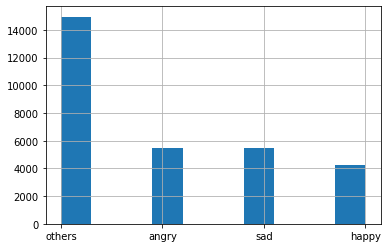
\includegraphics[width=8cm]{figures/rozklad_liczby_klas_semeval.png}
\fcmfcaption{Niezbalansowany rozkład etykiet emocji w danych z EmoContext.}\label{rys:rozklad_liczby_klas_semeval}
\end{figure}

Ostatnim elementem analizy eksploracyjnej tego zbioru jest identyfikacja najczęściej występujących \textit{N-gramów}, gdzie \textit{N} to liczba zlepek słów występujących obok siebie w dialogach. Rysunki \ref{rys:semeval_1_gram}, \ref{rys:semeval_2_gramy} oraz \ref{rys:semeval_3_gram} ukazują histogramy najczęstszych \textit{N-gramów}. Można zauważyć że najczęściej występującymi słowami są słowa należące do grupy słów nie wnoszących znaczenia (ang. \textit{stop words}), np.: słowa popularne, spójniki, przedimki, jednak często występujące słowa to także wnoszące dużo znaczenia do wypowiedzi takie jak \textit{love}, \textit{like}, \textit{good}, \textit{hate}.

\begin{figure}[t]
\centering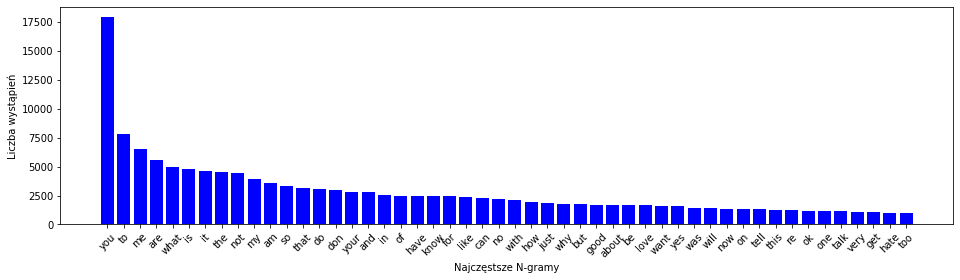
\includegraphics[width=\textwidth]{figures/semeval_1_gram.png}
\fcmfcaption{Rozkład wystąpień najczęstszych 1-gramów (wyrazów) w danych z EmoContext.}\label{rys:semeval_1_gram}
\end{figure}

\begin{figure}[t]
\centering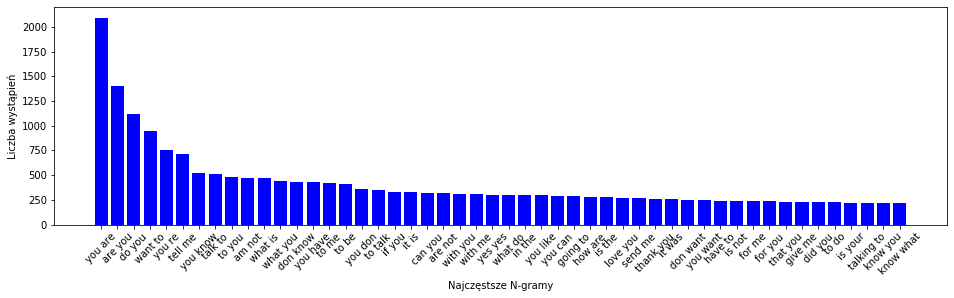
\includegraphics[width=\textwidth]{figures/semeval_2_gramy.png}
\fcmfcaption{Rozkład wystąpień najczęstszych 2-gramów w danych z EmoContext.}\label{rys:semeval_2_gramy}
\end{figure}

\begin{figure}[t]
\centering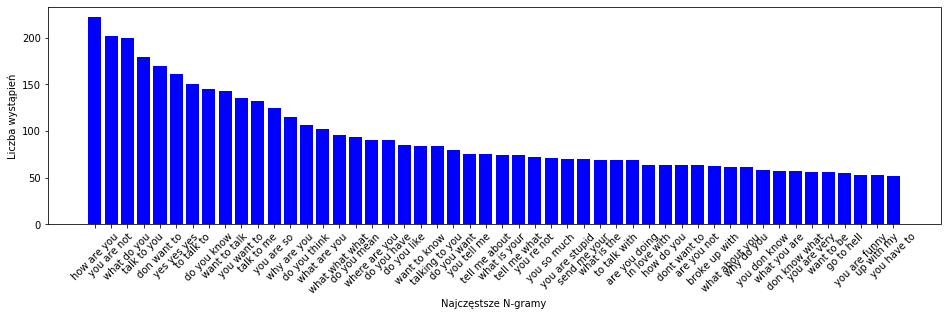
\includegraphics[width=\textwidth]{figures/semeval_3_gram.png}
\fcmfcaption{Rozkład wystąpień najczęstszych 3-gramów w danych z EmoContext.}\label{rys:semeval_3_gram}
\end{figure}
